\section{CAN}
\subsection{总线负载率计算}
标准数据帧的格式如图\ref{fig:can_frame}所示,
\begin{figure}[ht]
    \centering
    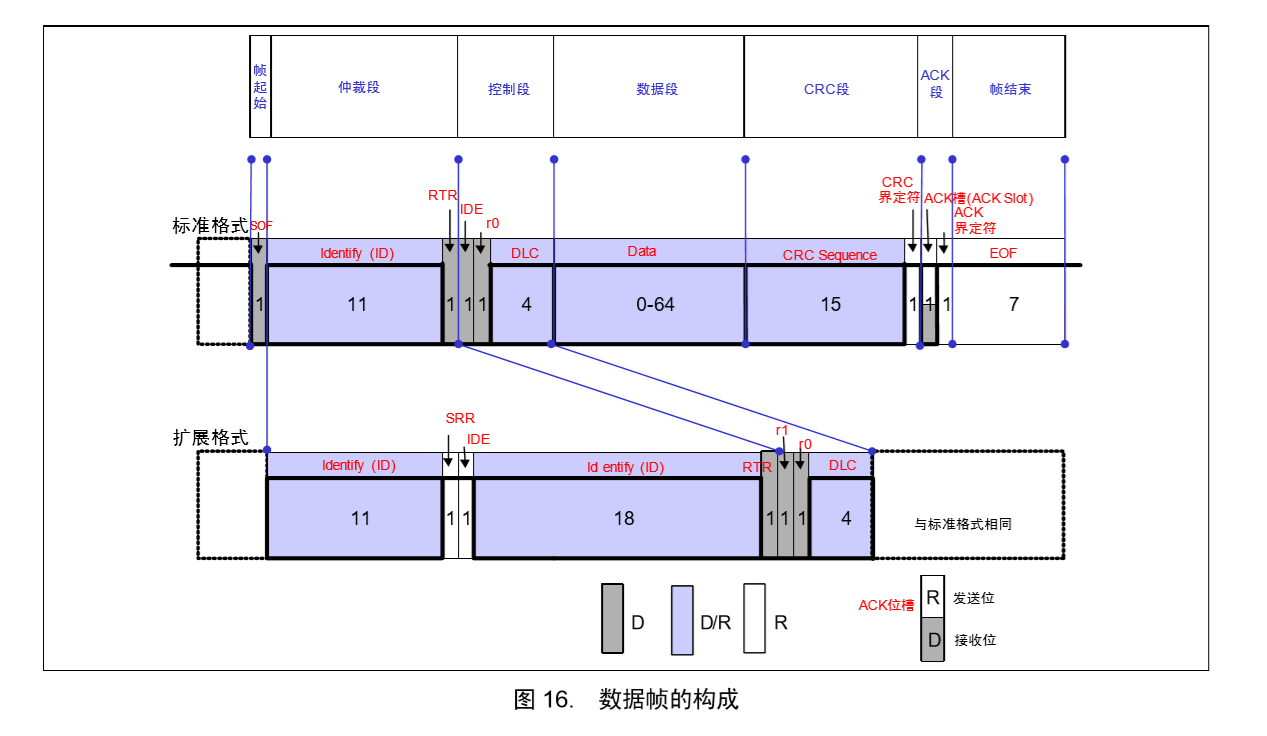
\includegraphics[scale=0.7]{pic/can_frame.png}
    \caption{CAN帧格式}
    \label{fig:can_frame}
\end{figure}

负载率由下式计算:
$$lr = \frac{1000}{T} \frac{len_{frame}}{bdrate} $$
其中,$T$为数据帧的发送周期(ms),$len_{frame}$为数据帧的长度(单位,bit),$bdrate$为总线波特率。

由图\ref{fig:can_frame},可知,在不考虑位填充和帧间隔的情况下,一个数据帧的长度$len_{frame}=64+34+10=108$,
假定周期为10ms的帧及500kbps的波特率,总线负载可得$lr=0.0216=2.16\%$。

位填充:为防止突发错误而设定的功能。当同样的电平持续 5 位时则添加一个位的反型数据。 
位填充在帧的SOF~CRC段进行。因此最大情况下,位填充为$\frac{34+64}{5}=19$。

帧间隔如图\ref{fig:frame_jiange}所示。
\begin{figure}[ht]
    \centering
    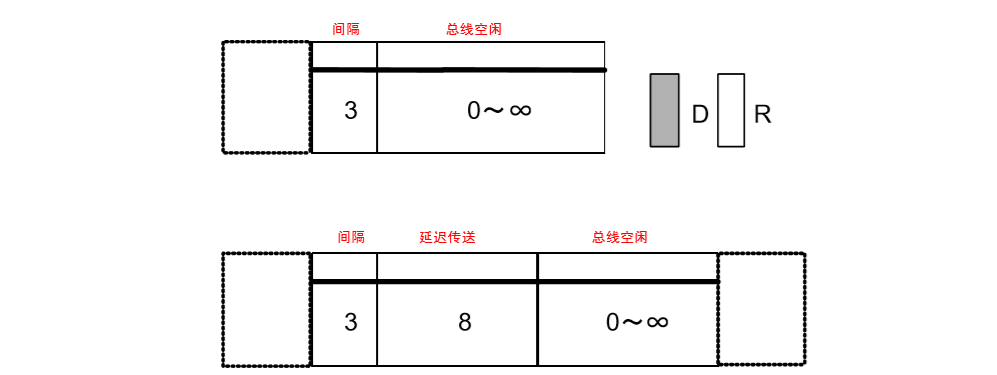
\includegraphics[]{pic/frame_jiange.png}
    \caption{帧间隔}
    \label{fig:frame_jiange}
\end{figure}

因此,最大帧长度$len_{frame}=34+64+10+19+3=130$,最大负载$lr=0.026=2.6\%$。
\section{UDSOnCAN}
\subsection{osi模型}
OSI七层模型:亦称OSI(Open System Interconnection)参考模型,是参考模型是国际标准化组织(ISO)制定的一个用于计算机或通信系统间互联的标准体系。

对USDonCan而言,如图\ref{fig:usd_oncan}所示,各层使用的标准如下:
\begin{figure}[ht]
    \centering
    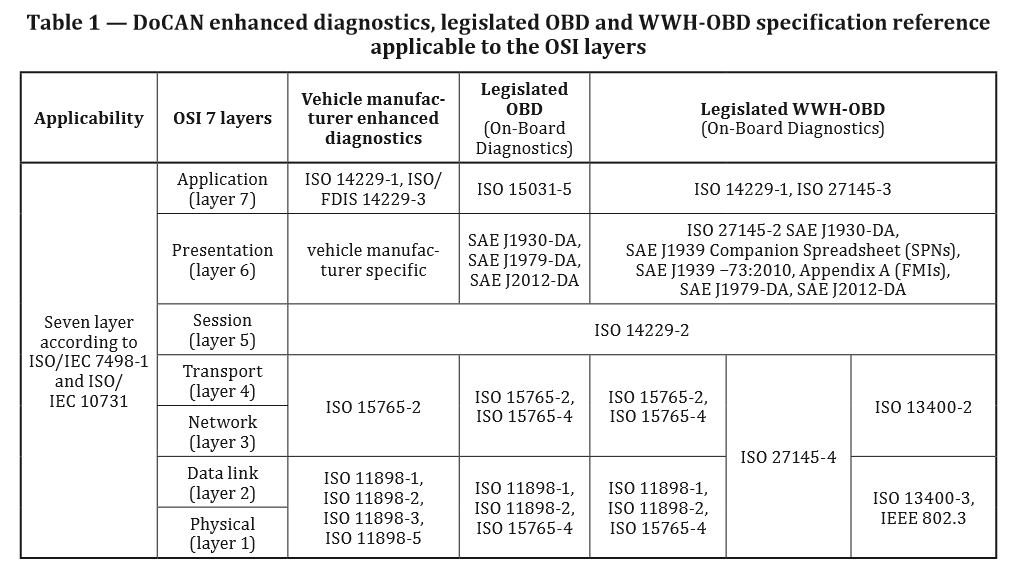
\includegraphics[]{pic/osi_uds_oncan.png}
    \caption{osi uds on can}
    \label{fig:usd_oncan}
\end{figure}
